% !TeX program = xelatex
\documentclass[a4paper,10pt]{article}

% ============================================================================
% ១. កញ្ចប់បណ្ណាល័យ និងការកំណត់ទំព័រ (Packages & Page Setup — តាមគំរូ ls_plan.tex)
% ============================================================================
\usepackage[a4paper, left=0.95cm, right=0.95cm, top=0.85cm, bottom=0.92cm, footskip=0.52cm]{geometry}
\usepackage{amsmath}
\usepackage{unicode-math}
\usepackage{fontspec}
\usepackage{longtable, array, multirow, colortbl}
\usepackage[table]{xcolor}
\usepackage{enumitem}
\usepackage{pifont}
\usepackage{fancyhdr}
\usepackage{tikz}
\usetikzlibrary{calc, arrows.meta, decorations.pathreplacing, patterns, positioning, babel}

\makeatletter
\let\@expl@@@mark@update@singlecol@structures@@\relax
\makeatother

% --- ប្រព័ន្ធស្វែងរកទីតាំងពុម្ពអក្សរស្វ័យប្រវត្តិ (Windows Local + Cloud Repo fonts/) ---
\providecommand{\NGSFindFonts}{%
  \IfFileExists{C:/Windows/Fonts/cambria.ttc}{%
    \def\NGSSysPath{C:/Windows/Fonts/}%
    \def\NGSUserPath{C:/Users/KIT/AppData/Local/Microsoft/Windows/Fonts/}%
  }{%
    \IfFileExists{./fonts/KhmerOSsiemreap.ttf}{\def\NGSSysPath{./fonts/}\def\NGSUserPath{./fonts/}}{%
    \IfFileExists{../fonts/KhmerOSsiemreap.ttf}{\def\NGSSysPath{../fonts/}\def\NGSUserPath{../fonts/}}{%
    \IfFileExists{../../fonts/KhmerOSsiemreap.ttf}{\def\NGSSysPath{../../fonts/}\def\NGSUserPath{../../fonts/}}{%
    \IfFileExists{../../../fonts/KhmerOSsiemreap.ttf}{\def\NGSSysPath{../../../fonts/}\def\NGSUserPath{../../../fonts/}}{%
    \IfFileExists{../../../../fonts/KhmerOSsiemreap.ttf}{\def\NGSSysPath{../../../../fonts/}\def\NGSUserPath{../../../../fonts/}}{%
    \IfFileExists{../../../../../fonts/KhmerOSsiemreap.ttf}{\def\NGSSysPath{../../../../../fonts/}\def\NGSUserPath{../../../../../fonts/}}{%
    \IfFileExists{../../../../../../fonts/KhmerOSsiemreap.ttf}{\def\NGSSysPath{../../../../../../fonts/}\def\NGSUserPath{../../../../../../fonts/}}{%
      \def\NGSSysPath{../../../../../../../fonts/}\def\NGSUserPath{../../../../../../../fonts/}%
    }}}}}}}%
  }%
}
\NGSFindFonts

% ============================================================================
% ២. កំណត់ពុម្ពអក្សរ (Fonts — តាមគំរូ ls_plan.tex)
% ============================================================================
\setmathfont[Path={\NGSSysPath}, FontIndex=1, Scale=1.02]{cambria.ttc}
\defaultfontfeatures{Ligatures=TeX}

\setmainfont[
  Path={\NGSUserPath},
  Extension=.ttf,
  Script=Khmer,
  BoldFont={KhmerOSsiemreap},
  BoldFeatures={FakeBold=1.8},
  ItalicFont={KhmerOSsiemreap},
  ItalicFeatures={FakeSlant=0.25},
  BoldItalicFont={KhmerOSsiemreap},
  BoldItalicFeatures={FakeBold=1.8, FakeSlant=0.25}
]{KhmerOSsiemreap}

\newfontfamily\muol[Path={\NGSUserPath}, Extension=.ttf, Script=Khmer]{KhmerOSmuollight}
\newfontfamily\Tacteing[Path={\NGSUserPath}, Extension=.TTF]{TACTENG}
\newfontfamily\TimesEn[Path={\NGSSysPath}, Extension=.ttf, BoldFont={timesbd}, ItalicFont={timesi}, BoldItalicFont={timesbi}]{times}
\newfontfamily\CalibriFont[Path={\NGSSysPath}, Extension=.ttf]{calibri}
\newfontfamily\CourierCirc[Path={\NGSSysPath}, Extension=.ttf]{cour}

\XeTeXlinebreaklocale "km"
\XeTeXlinebreakskip = 0pt plus 1pt minus 0.1pt

% ============================================================================
% ៣. ពណ៌ និងការតុបតែង (Colors & Styles)
% ============================================================================
\definecolor{stepbg}{HTML}{D9D9D9}
\definecolor{headgray}{HTML}{E6E6E6}
\definecolor{emphred}{HTML}{C00000}

\pagestyle{fancy}
\fancyhf{}
\renewcommand{\headrulewidth}{0pt}
\fancyfoot[R]{\CalibriFont\fontsize{9pt}{11pt}\selectfont\thepage}

\setlength{\parindent}{0pt}
\setlength{\parskip}{0pt}
\setlength{\tabcolsep}{4.5pt}
\setlength{\LTpre}{2pt}
\setlength{\LTpost}{2pt}

\newcolumntype{L}[1]{>{\raggedright\arraybackslash}p{#1}}
\newcolumntype{C}[1]{>{\centering\arraybackslash}p{#1}}

% ============================================================================
% ៤. ពាក្យបញ្ជាជំនួយ (Helper Macros)
% ============================================================================
\newcommand{\en}[1]{{\TimesEn #1}}
\newcommand{\enbf}[1]{{\TimesEn\bfseries #1}}
\newcommand{\khmflourish}{{\Tacteing\fontsize{15pt}{15pt}\selectfont 3}}
\newcommand{\wcirc}{{\CourierCirc\fontsize{9.5pt}{11pt}\selectfont o}}
\newcommand{\ditem}{{\fontsize{7.5pt}{10pt}\selectfont\ding{117}}\ }
\newcommand{\fiveE}[1]{\textcolor{emphred}{\CalibriFont\bfseries #1}}
\newcommand{\redsub}[1]{\textcolor{emphred}{#1}}
\newcommand{\timenote}[1]{\textcolor{emphred}{\textit{#1}}}
\newcommand{\stepheader}[1]{\multicolumn{3}{|c|}{\cellcolor{stepbg}\muol #1} \\ \hline}
\newcommand{\cfig}[1]{{\centering\vspace{3pt}#1\vspace{3pt}\par}}
\newcommand{\cnum}[1]{\mbox{\fontsize{10.5pt}{12pt}\selectfont\ding{\numexpr181+#1\relax}}}
\newcommand{\unit}[1]{\,\text{\en{#1}}}
\newcommand{\graybox}[1]{\colorbox{headgray}{\strut #1}}

% ============================================================================
% ៥. រូបភាព TikZ ស-ខ្មៅ សម្រាប់បង្រៀនលើក្ដារខៀន និងសន្លឹកកិច្ចការ (B&W Diagrams)
% ============================================================================

% ១. E1 Engage: អន្ទាក់ឈប់ត្រឹមកត្តាមិនបឋម 36 = 4 x 9 vs 2^2 x 3^2
\newcommand{\figEngageDIVTwoFour}{%
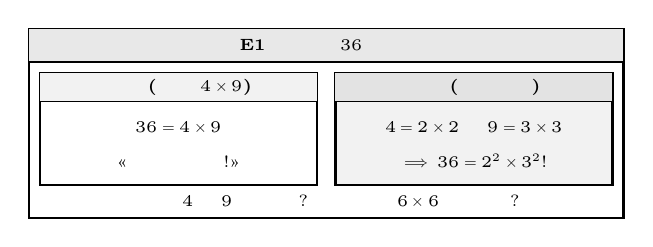
\begin{tikzpicture}[x=1cm, y=1cm, every node/.style={font=\fontsize{5.9pt}{7.8pt}\selectfont, text=black}]
  \draw[black, line width=0.9pt] (0,0) rectangle (7.55,2.40);
  \fill[gray!18] (0,1.98) rectangle (7.55,2.40);
  \draw[black, line width=0.6pt] (0,1.98) -- (7.55,1.98);
  \node at (3.775,2.19) {\textbf{បេសកកម្ម \en{E1}៖ អន្ទាក់បំបែក $36$ ឈប់ត្រឹមកត្តាមិនបឋម}};

  % Student A
  \draw[black, line width=0.8pt] (0.14,0.42) rectangle (3.66,1.84);
  \fill[gray!10] (0.14,1.48) rectangle (3.66,1.84);
  \draw[black, line width=0.5pt] (0.14,1.48) -- (3.66,1.48);
  \node at (1.90,1.66) {\textbf{សិស្ស ក (ឈប់ត្រឹម $4 \times 9$)}};
  \node at (1.90,1.15) {$36 = 4 \times 9$};
  \node at (1.90,0.72) {«បំបែកជាកត្តាបឋមរួចហើយ!»};

  % Student B
  \draw[black, line width=0.95pt, fill=gray!10] (3.89,0.42) rectangle (7.41,1.84);
  \fill[gray!22] (3.89,1.48) rectangle (7.41,1.84);
  \draw[black, line width=0.55pt] (3.89,1.48) -- (7.41,1.48);
  \node at (5.65,1.66) {\textbf{សិស្ស ខ (បំបែកដល់ចំនួនបឋម)}};
  \node at (5.65,1.15) {$4=2\times 2$ និង $9=3\times 3$};
  \node at (5.65,0.72) {$\implies 36 = 2^2 \times 3^2$!};

  \node at (3.775,0.21) {\textbf{សំណួរ៖} តើ $4$ និង $9$ ជាចំនួនបឋមឬទេ? ហើយបើចាប់ផ្ដើមពី $6\times 6$ តើបានដូចគ្នាទេ?};
\end{tikzpicture}}

% ២. E2 Explore: វិធីទី 1 (ចែកឈរ) និង វិធីទី 2 (ដ្យាក្រាមដើមឈើ) លើចំនួន 30 (ទំ.២០)
\newcommand{\figTwoMethodsDIVTwoFour}{%
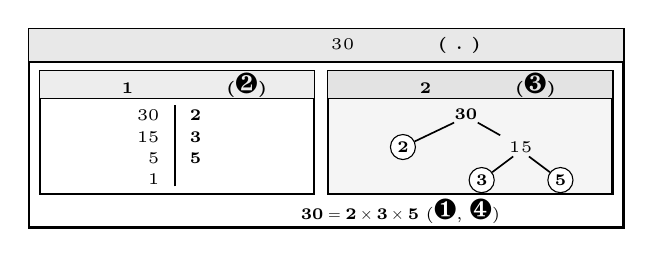
\begin{tikzpicture}[x=1cm, y=1cm, every node/.style={font=\fontsize{5.9pt}{7.7pt}\selectfont, text=black}]
  \draw[black, line width=0.9pt] (0,0) rectangle (7.55,2.52);
  \fill[gray!18] (0,2.10) rectangle (7.55,2.52);
  \draw[black, line width=0.6pt] (0,2.10) -- (7.55,2.10);
  \node at (3.775,2.31) {\textbf{ប្រៀបធៀបវិធីទាំង ២ ក្នុងការបំបែក $30$ ជាផលគុណកត្តាបឋម (ទំ.២០)}};

  % Left: Vertical Prime Division Ladder
  \draw[black, line width=0.8pt] (0.14,0.42) rectangle (3.62,1.98);
  \fill[gray!14] (0.14,1.64) rectangle (3.62,1.98);
  \draw[black, line width=0.5pt] (0.14,1.64) -- (3.62,1.64);
  \node at (1.88,1.81) {\textbf{វិធីទី 1៖ ចែកឈរបន្តបន្ទាប់ (\cnum{2})}};
  \draw[black, line width=0.7pt] (1.85,0.52) -- (1.85,1.56);
  \node[anchor=east] at (1.78,1.42) {$30$}; \node[anchor=west] at (1.92,1.42) {$\mathbf{2}$};
  \node[anchor=east] at (1.78,1.15) {$15$}; \node[anchor=west] at (1.92,1.15) {$\mathbf{3}$};
  \node[anchor=east] at (1.78,0.88) {$5$};  \node[anchor=west] at (1.92,0.88) {$\mathbf{5}$};
  \node[anchor=east] at (1.78,0.61) {$1$};

  % Right: Factor Tree
  \draw[black, line width=0.85pt, fill=gray!8] (3.80,0.42) rectangle (7.41,1.98);
  \fill[gray!22] (3.80,1.64) rectangle (7.41,1.98);
  \draw[black, line width=0.5pt] (3.80,1.64) -- (7.41,1.64);
  \node at (5.605,1.81) {\textbf{វិធីទី 2៖ ដ្យាក្រាមដើមឈើ (\cnum{3})}};
  \node at (5.55,1.44) {$\mathbf{30}$};
  \node[draw=black, circle, inner sep=1.2pt, fill=white] (p2) at (4.75,1.02) {$\mathbf{2}$};
  \node (c15) at (6.25,1.02) {$15$};
  \node[draw=black, circle, inner sep=1.2pt, fill=white] (p3) at (5.75,0.60) {$\mathbf{3}$};
  \node[draw=black, circle, inner sep=1.2pt, fill=white] (p5) at (6.75,0.60) {$\mathbf{5}$};
  \draw[black, line width=0.6pt] (5.40,1.33) -- (p2);
  \draw[black, line width=0.6pt] (5.70,1.33) -- (c15);
  \draw[black, line width=0.6pt] (6.15,0.90) -- (p3);
  \draw[black, line width=0.6pt] (6.35,0.90) -- (p5);

  \node at (3.775,0.21) {វិធីទាំងពីរផ្ដល់លទ្ធផលតែមួយគត់៖ $\mathbf{30 = 2 \times 3 \times 5}$ (\cnum{1}, \cnum{4})};
\end{tikzpicture}}

% ៣. E4 Elaborate: លំហាត់គំរូ ទំ.២០ (x=180, y=360 និង x+y=540)
\newcommand{\figModelsDIVTwoFour}{%
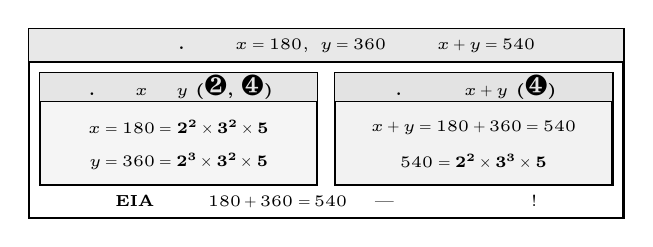
\begin{tikzpicture}[x=1cm, y=1cm, every node/.style={font=\fontsize{5.8pt}{7.6pt}\selectfont, text=black}]
  \draw[black, line width=0.9pt] (0,0) rectangle (7.55,2.40);
  \fill[gray!18] (0,1.98) rectangle (7.55,2.40);
  \draw[black, line width=0.6pt] (0,1.98) -- (7.55,1.98);
  \node at (3.775,2.19) {\textbf{លំហាត់គំរូ ទំ.២០៖ បំបែក $x=180,\ y=360$ និងផលបូក $x+y=540$}};

  % Left: x=180 and y=360
  \draw[black, line width=0.85pt, fill=gray!8] (0.14,0.42) rectangle (3.66,1.84);
  \fill[gray!20] (0.14,1.48) rectangle (3.66,1.84);
  \draw[black, line width=0.5pt] (0.14,1.48) -- (3.66,1.48);
  \node at (1.90,1.66) {\textbf{ក. បំបែក $x$ និង $y$ (\cnum{2}, \cnum{4})}};
  \node at (1.90,1.15) {$x = 180 = \mathbf{2^2 \times 3^2 \times 5}$};
  \node at (1.90,0.72) {$y = 360 = \mathbf{2^3 \times 3^2 \times 5}$};

  % Right: x + y = 540
  \draw[black, line width=0.85pt, fill=gray!10] (3.89,0.42) rectangle (7.41,1.84);
  \fill[gray!22] (3.89,1.48) rectangle (7.41,1.84);
  \draw[black, line width=0.5pt] (3.89,1.48) -- (7.41,1.48);
  \node at (5.65,1.66) {\textbf{ខ. បំបែកផលបូក $x+y$ (\cnum{4})}};
  \node at (5.65,1.15) {$x + y = 180 + 360 = 540$};
  \node at (5.65,0.72) {$540 = \mathbf{2^2 \times 3^3 \times 5}$};

  \node at (3.775,0.21) {\textbf{\en{EIA}៖} ត្រូវបូក $180+360=540$ សិន — ហាមបូកនិទស្សន្តលើផលបូកដាច់ខាត!};
\end{tikzpicture}}

% ៣ខ. E5 Practice: ប្រតិបត្តិ ទំ.២០ (66 និង 273)
\newcommand{\figPracticeDIVTwoFour}{%
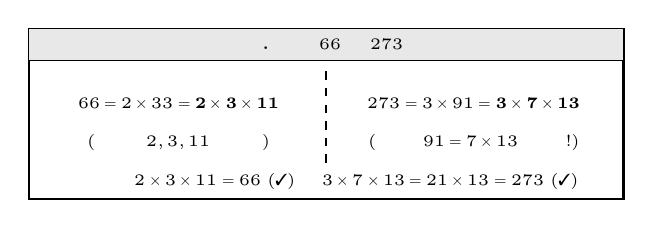
\begin{tikzpicture}[x=1cm, y=1cm, every node/.style={font=\fontsize{5.8pt}{7.6pt}\selectfont, text=black}]
  \draw[black, line width=0.9pt] (0,0) rectangle (7.55,2.16);
  \fill[gray!18] (0,1.76) rectangle (7.55,2.16);
  \draw[black, line width=0.6pt] (0,1.76) -- (7.55,1.76);
  \node at (3.775,1.96) {\textbf{លំហាត់ប្រតិបត្តិ ទំ.២០៖ បំបែក $66$ និង $273$ ជាផលគុណកត្តាបឋម}};
  \node at (1.90,1.22) {$66 = 2 \times 33 = \mathbf{2 \times 3 \times 11}$};
  \node at (1.90,0.72) {(គ្រប់កត្តា $2, 3, 11$ សុទ្ធតែបឋម)};
  \draw[black, dashed, line width=0.5pt] (3.775,0.46) -- (3.775,1.66);
  \node at (5.65,1.22) {$273 = 3 \times 91 = \mathbf{3 \times 7 \times 13}$};
  \node at (5.65,0.72) {(ប្រយ័ត្ន៖ $91 = 7\times 13$ មិនមែនបឋម!)};
  \node at (3.775,0.22) {ផ្ទៀងផ្ទាត់៖ $2\times 3\times 11 = 66$ (\ding{51}) និង $3\times 7\times 13 = 21\times 13 = 273$ (\ding{51})};
\end{tikzpicture}}

% ៤. E5 Evaluate: សំណួរវិនិច្ឆ័យ A-D
\newcommand{\figExitDIVTwoFour}{%
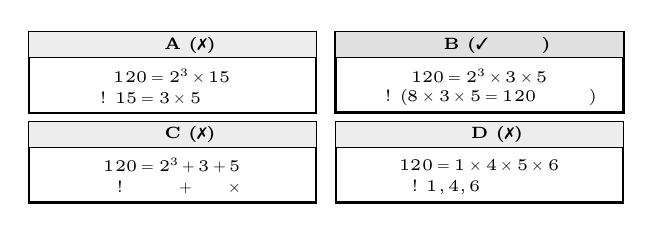
\begin{tikzpicture}[x=1cm, y=1cm, every node/.style={font=\fontsize{5.9pt}{7.6pt}\selectfont, text=black}]
  % Choice A
  \draw[black, line width=0.8pt] (0,1.14) rectangle (3.65,2.16);
  \fill[gray!14] (0,1.84) rectangle (3.65,2.16);
  \draw[black, line width=0.5pt] (0,1.84) -- (3.65,1.84);
  \node at (1.825,2.00) {\textbf{ជម្រើស \en{A} (\ding{55})}};
  \node at (1.825,1.61) {$120 = 2^3 \times 15$};
  \node at (1.825,1.33) {ខុស! $15 = 3\times 5$ មិនមែនបឋមទេ};

  % Choice B (Correct)
  \draw[black, line width=1.05pt] (3.90,1.14) rectangle (7.55,2.16);
  \fill[gray!24] (3.90,1.84) rectangle (7.55,2.16);
  \draw[black, line width=0.6pt] (3.90,1.84) -- (7.55,1.84);
  \node at (5.725,2.00) {\textbf{ជម្រើស \en{B} (\ding{51} ត្រឹមត្រូវ)}};
  \node at (5.725,1.61) {$120 = 2^3 \times 3 \times 5$};
  \node at (5.725,1.33) {ត្រូវ! ($8\times 3\times 5 = 120$ បឋមទាំងអស់)};

  % Choice C
  \draw[black, line width=0.8pt] (0,0) rectangle (3.65,1.02);
  \fill[gray!14] (0,0.70) rectangle (3.65,1.02);
  \draw[black, line width=0.5pt] (0,0.70) -- (3.65,0.70);
  \node at (1.825,0.86) {\textbf{ជម្រើស \en{C} (\ding{55})}};
  \node at (1.825,0.47) {$120 = 2^3 + 3 + 5$};
  \node at (1.825,0.19) {ខុស! ប្រើសញ្ញា $+$ ជំនួស $\times$};

  % Choice D
  \draw[black, line width=0.8pt] (3.90,0) rectangle (7.55,1.02);
  \fill[gray!14] (3.90,0.70) rectangle (7.55,1.02);
  \draw[black, line width=0.5pt] (3.90,0.70) -- (7.55,0.70);
  \node at (5.725,0.86) {\textbf{ជម្រើស \en{D} (\ding{55})}};
  \node at (5.725,0.47) {$120 = 1 \times 4 \times 5 \times 6$};
  \node at (5.725,0.19) {ខុស! $1, 4, 6$ មិនមែនចំនួនបឋមទេ};
\end{tikzpicture}}

\begin{document}
\fontsize{10pt}{15.2pt}\selectfont

% ============================================================================
% ក្បាលរដ្ឋបាល (Administrative Header — តាមគំរូ ls_plan.tex)
% ============================================================================
{\centering
  {\muol\fontsize{11pt}{16pt}\selectfont ព្រះរាជាណាចក្រកម្ពុជា\par}
  {\muol\fontsize{11pt}{16pt}\selectfont ជាតិ សាសនា ព្រះមហាក្សត្រ\par}
  \vspace{-3pt}{\khmflourish\par}
}

\vspace{1pt}
{\muol\fontsize{10pt}{15.5pt}\selectfont
មន្ទីរអប់រំ យុវជន និងកីឡា ខេត្តកំពង់ធំ\par
ការិយាល័យអប់រំ យុវជន និងកីឡា ស្រុកកំពង់ស្វាយ\par
អនុវិទ្យាល័យព្រះក្រសាំង\par}

\vspace{2pt}
{\centering{\muol\fontsize{11.5pt}{17pt}\selectfont កិច្ចតែងការបង្រៀន\par}}
\vspace{2pt}

% --- ព័ត៌មានទូទៅ ---
{\hspace*{2.8cm}\renewcommand{\arraystretch}{1.08}
\begin{tabular}{@{}l@{\hspace{0.35cm}}p{2.9cm}@{\hspace{0.15cm}}c@{\hspace{0.25cm}}l@{}}
  - & មុខវិជ្ជា & : & គណិតវិទ្យា ថ្នាក់ទី៧ (ពីជគណិត) \\
  - & ចំណងជើងមេរៀន & : & មេរៀនទី២៖ តួចែកនិងពហុគុណ \\
  - & ចំណងជើងរង & : & ៤. ការបំបែកមួយចំនួនជាផលគុណកត្តាបឋម (សៀវភៅគោល ទំ.២០) \\
  - & រយៈពេល & : & ១ ម៉ោងសិក្សា (៥០ នាទី) \\
  - & បង្រៀនដោយ & : & ហុក ប៊ុនថែន \\
  - & កាលបរិច្ឆេទ & : & ថ្ងៃចន្ទ ទី១៦ ខែវិច្ឆិកា ឆ្នាំ២០២៦ \\
\end{tabular}\par}

\vspace{2pt}

% --- I. វត្ថុបំណង ---
{\muol\fontsize{10pt}{15.5pt}\selectfont \enbf{I.} វត្ថុបំណង\par}
\vspace{1pt}
{\renewcommand{\arraystretch}{1.10}
\begin{tabular}{@{}p{0.55cm}@{}p{2.35cm}@{\hspace{0.15cm}}c@{\hspace{0.25cm}}p{14.95cm}@{}}
  \hfill\wcirc\hspace{0.2cm} & វិជ្ជាសម្បទា & : & សិស្សប្រាប់បានពីអត្ថន័យនិងវិធីទាំងពីរ (ចែកឈរបន្តបន្ទាប់ និងដ្យាក្រាមដើមឈើ) នៃការបំបែកចំនួនមិនបឋមជាផលគុណកត្តាបឋមបានត្រឹមត្រូវ (ទំ.២០) ។ \\
  \hfill\wcirc\hspace{0.2cm} & បំណិនសម្បទា & : & សិស្សបំបែកចំនួនគត់ធម្មជាតិជាផលគុណកត្តាបឋមក្នុងទម្រង់ស្វ័យគុណតាមលំដាប់កើនលើសន្លឹកកិច្ចការបានត្រឹមត្រូវ ។ \\
  \hfill\wcirc\hspace{0.2cm} & ចរិយាសម្បទា & : & សិស្សមានភាពម៉ត់ចត់បំបែករហូតអស់កត្តាមិនបឋម គុណផ្ទៀងផ្ទាត់ចម្លើយឡើងវិញ និងសហការពិភាក្សាជាក្រុមដោយសកម្ម ។ \\
\end{tabular}\par}

\vspace{2pt}

% --- II. សម្ភារៈឧបទេស ---
{\muol\fontsize{10pt}{15.5pt}\selectfont \enbf{II.} សម្ភារៈឧបទេស\par}
\vspace{1pt}
\hspace*{0.55cm}$\bullet$\ សៀវភៅសិក្សាគោលថ្នាក់ទី៧ (ទំ.២០ និងទំ.២៤) ក្ដារខៀន ដីស/ហ្វឺត និង\textbf{សន្លឹកកិច្ចការសិស្សបំពេញចន្លោះ ស-ខ្មៅ} (កូដ \en{DIV24} ទំព័រ ១--២ សម្រាប់សិស្ស និងទំព័រ ៣ ប្លង់ក្ដារខៀន/ចម្លើយគ្រូ — គ្មានប្រើ \en{LCD})\par

\vspace{2pt}

% --- III. វិធីសាស្រ្តបង្រៀន ---
{\muol\fontsize{10pt}{15.5pt}\selectfont \enbf{III.} វិធីសាស្រ្តបង្រៀន\par}
\vspace{1pt}
{\renewcommand{\arraystretch}{1.08}
\begin{tabular}{@{}p{0.55cm}@{}p{2.35cm}@{\hspace{0.15cm}}c@{\hspace{0.25cm}}p{14.95cm}@{}}
  \hfill$\bullet$\hspace{0.2cm} & គោលវិធី & : & សិស្សមជ្ឈមណ្ឌល (សន្លឹកកិច្ចការបំពេញចន្លោះជាគោល + ការពិភាក្សាជាក្រុមតូច ៣ នាក់) \\
  \hfill$\bullet$\hspace{0.2cm} & យុទ្ធវិធីបង្រៀន & : & គំរូស្ថាបនានិយម \en{5Es} រួមបញ្ចូល \textbf{ការប្រៀបធៀបទន្ទឹមគ្នារវាងចែកឈរ និងដ្យាក្រាមដើមឈើ (\en{Dual-Representation Comparison})} \\
\end{tabular}\par}

\vspace{2pt}

% --- IV. ដំណើរការបង្រៀន ---
{\muol\fontsize{10pt}{15.5pt}\selectfont \enbf{IV.} ដំណើរការបង្រៀន\par}

{\renewcommand{\arraystretch}{1.14}
\begin{longtable}{|L{5.50cm}|L{7.90cm}|L{4.80cm}|}
\hline
\multicolumn{1}{|c|}{\cellcolor{headgray}\muol សកម្មភាពគ្រូ} &
\multicolumn{1}{c|}{\cellcolor{headgray}\muol ខ្លឹមសារមេរៀន} &
\multicolumn{1}{c|}{\cellcolor{headgray}\muol សកម្មភាពសិស្ស} \\
\hline
\endfirsthead

\hline
\multicolumn{1}{|c|}{\cellcolor{headgray}\muol សកម្មភាពគ្រូ} &
\multicolumn{1}{c|}{\cellcolor{headgray}\muol ខ្លឹមសារមេរៀន} &
\multicolumn{1}{c|}{\cellcolor{headgray}\muol សកម្មភាពសិស្ស} \\
\hline
\endhead

% ==================== ជំហានទី១ (2min) ====================
\stepheader{ជំហានទី១ \enbf{(}រដ្ឋបាលថ្នាក់\enbf{)}}
$\bullet$ ពិនិត្យវត្តមាន អនាម័យ និងសណ្ដាប់ធ្នាប់ថ្នាក់រៀន \par
$\bullet$ រៀបចំក្រុមតូច ៣ នាក់តាមតុ និងចែក\textbf{សន្លឹកកិច្ចការសិស្ស (\en{DIV24} ទំព័រ ១–២)}
&
$\bullet$ រដ្ឋបាលថ្នាក់ អនាម័យ និងវិន័យសិក្សា \par
$\bullet$ ចែកសន្លឹកកិច្ចការម្នាក់ ១ សន្លឹក សម្រាប់បំពេញតាមដំណាក់កាល \en{E1--E5}
&
$\circ$ ប្រធានថ្នាក់រាយការណ៍វត្តមានសិស្ស \par
$\circ$ ទទួលសន្លឹកកិច្ចការ សរសេរឈ្មោះ និងអង្គុយតាមក្រុម ៣ នាក់ \\
\hline

% ==================== ជំហានទី២ (9min: កំណែ <=3m + រំលឹក 3m + E1 3m) ====================
\stepheader{ជំហានទី២ \enbf{(}កិច្ចការផ្ទះ \enbf{+} ទំនាក់ទំនងមេរៀនថ្មី\enbf{)}}
\ditem \textbf{កំណែកិច្ចការផ្ទះ ($\le\text{\enbf{3\,min}}$)} \par
$\bullet$ ហៅសិស្សផ្ទៀងផ្ទាត់ចម្លើយលំហាត់ទំ.២៤ លេខ ៤ (ក, ខ) លើក្ដារខៀនឆ្វេង
&
{\centering\redsub{កំណែកិច្ចការផ្ទះមេរៀនមុន (ទំ.២៤ លេខ ៤)}\par}
$\bullet$ \textbf{ក. តួចែក៖} $15:\{1,3,5,15\}$, $18:\{1,2,3,6,9,18\}$, $21:\{1,3,7,21\}$, \dots \par
$\bullet$ \textbf{ខ. ចំនួនបឋម៖} គឺចំនួនមានតួចែកតែពីរគត់៖ $\mathbf{11,\ 17,\ 19,\ 23,\ 29}$
&
$\circ$ ផ្ទៀងចម្លើយលេខ ៤ និងកែចូលសៀវភៅ \\[3pt]

\ditem \textbf{រំលឹកមេរៀនទាក់ទង (\enbf{3min})} \par
$\bullet$ សួរ៖ «ចូររាយចំនួនបឋម ៦ តួដំបូងពីតូចទៅធំ និងសរសេរ $2\times 2\times 2\times 3\times 3$ ជាស្វ័យគុណ!»
&
{\centering\redsub{រំលឹកចំនួនបឋមតូចៗ និងស្វ័យគុណ}\par}
$\bullet$ ចំនួនបឋម ៦ តួដំបូង៖ $\mathbf{2,\ 3,\ 5,\ 7,\ 11,\ 13}$ \par
$\bullet$ $2\times 2\times 2\times 3\times 3 = \mathbf{2^3 \times 3^2}$
&
$\circ$ ឆ្លើយរាយបឋម $2, 3, 5, 7, 11, 13$ និងសរសេរ $2^3\times 3^2$ \\[3pt]

\fiveE{E1 - Engage (3min)} \timenote{(កុំទាន់ផ្ដល់ចម្លើយ)} \par
\ditem \textbf{បេសកកម្មអន្ទាក់ឈប់ត្រឹមកត្តាមិនបឋម (\en{E1})}
&
\redsub{បេសកកម្ម \en{E1}៖ តើអ្នកណាបំបែក $36$ ជាផលគុណកត្តាបឋមបានត្រឹមត្រូវ?}
&
$\circ$ អានស្ថានភាពបញ្ហា \en{E1} \\[3pt]

$\bullet$ ឱ្យសិស្សពិភាក្សាជាគូលើសន្លឹកកិច្ចការ \en{E1} រវាងសិស្ស ក ($4\times 9$) និងសិស្ស ខ ($2^2\times 3^2$)
&
$\bullet$ \textbf{សិស្ស ក៖} «$36 = 4 \times 9$ — បំបែកជាផលគុណកត្តាបឋមរួចហើយ!» \par
$\bullet$ \textbf{សិស្ស ខ៖} «$4$ និង $9$ មិនទាន់បឋមទេ ត្រូវបំបែកបន្តបាន $36 = 2^2 \times 3^2$!»
&
$\circ$ ពិភាក្សាជាគូ និងគូស \ding{51} ក្នុងប្រអប់ \en{E1} \\[3pt]

&
\cfig{\figEngageDIVTwoFour}
& \\
\hline

% ==================== ជំហានទី៣ (17min: E2 11m + E3 6m) ====================
\stepheader{ជំហានទី៣ \enbf{(}ខ្លឹមសារមេរៀនថ្មី\enbf{)}}
\fiveE{E2 - Explore (11min)} \par
$\bullet$ សរសេរចំណងជើងរង \textbf{៤. ការបំបែកមួយចំនួនជាផលគុណកត្តាបឋម} \par
\ditem \textbf{សកម្មភាព ១៖ ប្រៀបធៀបវិធីទី 1 និងវិធីទី 2 លើចំនួន $30$ (ទំ.២០, \enbf{5.5min}, \en{E2-A})}
&
៤. ការបំបែកមួយចំនួនជាផលគុណកត្តាបឋម (ទំ.២០) \par
$\bullet$ \textbf{ឧទាហរណ៍ ១ (បំបែក $30$)៖} \par
\hspace*{0.15cm}-- \textbf{វិធីទី 1 (ចែកឈរ)៖} $30\div 2=15 \to 15\div 3=5 \to 5\div 5=1 \implies 30 = 2\times 3\times 5$
&
$\circ$ បំពេញការចែកឈរនៃ $30$ នឹងបឋម $2, 3, 5$ លើ \en{E2-A} \\[3pt]

$\bullet$ ឱ្យសិស្សបំបែក $30$ តាម\textbf{វិធីទី 2 (ដ្យាក្រាមដើមឈើ)} និងសាកល្បងបែកមែកផ្សេង ($5\times 6$)
&
\hspace*{0.15cm}-- \textbf{វិធីទី 2 (ដ្យាក្រាមដើមឈើ)៖} $30 = 2\times 15 = 2\times 3\times 5$ (ឬ $30 = 5\times 6 = 5\times 2\times 3 = 2\times 3\times 5$) — ទោះបែកមែកបែបណា ក៏បានកត្តាបឋមដូចគ្នា!
&
$\circ$ គូសរង្វង់ចុងមែកបឋម ឃើញបាន $2\times 3\times 5$ ដូចគ្នា \\[3pt]

\ditem \textbf{សកម្មភាព ២៖ ការបំបែកចំនួនមានកត្តាបឋមស្ទួនជាស្វ័យគុណ (\enbf{5.5min}, \en{E2-B})} \par
$\bullet$ ឱ្យសិស្សបំបែក $72$ ទាំងតាមចែកឈរ និងដើមឈើ រួចសរសេរជាស្វ័យគុណ
&
$\bullet$ \textbf{ឧទាហរណ៍ ២ (បំបែក $72$)៖} $72\div 2=36\div 2=18\div 2=9\div 3=3\div 3=1$ \par
$\implies 72 = 2\times 2\times 2\times 3\times 3 = \mathbf{2^3 \times 3^2}$
&
$\circ$ បំបែក $72$ និងបង្រួមកត្តាដូចគ្នាជា $2^3\times 3^2$ \\[3pt]

&
\cfig{\figTwoMethodsDIVTwoFour}
& \\[3pt]

% --- E3 Explain (6min) ---
\fiveE{E3 - Explain (6min)} \par
$\bullet$ ដឹកនាំសិស្សសង្ខេបវិធានទូទៅ (ទំ.២០) លើសន្លឹកកិច្ចការ \en{E3}
&
$\bullet$ \textbf{ជាទូទៅ (ទំ.២០)៖} គ្រប់ចំនួនមិនបឋមទាំងអស់ អាចសរសេរជា\graybox{ផលគុណនៃកត្តាបឋម} បានតែមួយបែបគត់ (បើរៀបកត្តាបឋមពីតូចទៅធំ) ។
&
$\circ$ បំពេញប្រអប់សង្ខេបវិធានទូទៅលើ \en{E3} \\[3pt]

$\bullet$ ពន្យល់\textbf{សម្គាល់អំពីចំនួន $1$} ក្នុងផលគុណកត្តាបឋម
&
$\bullet$ \textbf{សម្គាល់៖} គេ\textbf{មិនដាក់ $1$} ក្នុងផលគុណកត្តាបឋមឡើយ ព្រោះ $1$ មិនមែនជាចំនួនបឋម (បើដាក់ $1$ នឹងធ្វើឱ្យមានច្រើនបែបដូចជា $1\times 30 = 1^2\times 30$) ។
&
$\circ$ កត់សម្គាល់មិនដាក់ $1$ ជាកត្តាបឋមដាច់ខាត \\[3pt]

$\bullet$ ភ្ជាប់\textbf{ធនាគារហេតុផល \cnum{1}} (លក្ខខណ្ឌកត្តាបឋម)
&
\textbf{ធនាគារហេតុផល (\en{Warrant Bank})៖} \par
\cnum{1} \textbf{លក្ខខណ្ឌកត្តាបឋម៖} គ្រប់កត្តាចុងក្រោយត្រូវតែជាចំនួនបឋម ភ្ជាប់ដោយសញ្ញា $\times$
&
$\circ$ ផ្ទៀងលេខកូដ \cnum{1} លើសន្លឹកកិច្ចការ \\[3pt]

$\bullet$ ភ្ជាប់\textbf{ធនាគារហេតុផល \cnum{2}} (វិធីទី 1៖ ចែកឈរបន្តបន្ទាប់)
&
\cnum{2} \textbf{វិធីទី 1 (ចែកឈរ)៖} ចែកបន្តបន្ទាប់នឹងបឋមពីតូចទៅធំ ($2, 3, 5, 7, \dots$) រហូតផលចែកស្មើ $1$
&
$\circ$ ផ្ទៀងលេខកូដ \cnum{2} លើសន្លឹកកិច្ចការ \\[3pt]

$\bullet$ ភ្ជាប់\textbf{ធនាគារហេតុផល \cnum{3}} (វិធីទី 2៖ ដ្យាក្រាមដើមឈើ)
&
\cnum{3} \textbf{វិធីទី 2 (ដើមឈើ)៖} បែកមែកផលគុណរហូតគ្រប់ចុងមែកជាចំនួនបឋម (គូសរង្វង់ចុងមែក)
&
$\circ$ ផ្ទៀងលេខកូដ \cnum{3} លើសន្លឹកកិច្ចការ \\[3pt]

$\bullet$ ភ្ជាប់\textbf{ធនាគារហេតុផល \cnum{4}} (ទម្រង់ស្វ័យគុណ និងផ្ទៀងផ្ទាត់)
&
\cnum{4} \textbf{ទម្រង់ស្វ័យគុណ៖} ប្រមូលកត្តាដូចគ្នាជាស្វ័យគុណតាមលំដាប់កើន រួចគុណផ្ទៀងផ្ទាត់ឡើងវិញ
&
$\circ$ ផ្ទៀងលេខកូដ \cnum{4} លើសន្លឹកកិច្ចការ \\
\hline

% ==================== ជំហានទី៤ (20min: E4 10m + E5 10m) ====================
\stepheader{ជំហានទី៤ \enbf{(}ពង្រីកចំណេះដឹង\enbf{)}}
\fiveE{E4 - Elaborate (10min)} \par
\ditem \textbf{លំហាត់គំរូ ក និង ខ តាមសៀវភៅគោល ទំ.២០ ($x=180,\ y=360$)}
&
{\muol លំហាត់គំរូ} \textbf{(សៀវភៅគោល ទំ.២០ — គេឱ្យ $x=180$ និង $y=360$)៖}
&
$\circ$ អានប្រធានលំហាត់គំរូទំ.២០ \\[3pt]

$\bullet$ ឱ្យសិស្សបំបែក $x=180$ តាមចែកឈរលើសន្លឹកកិច្ចការ \en{E4}
&
$\bullet$ \textbf{ក. បំបែក $x=180$៖} $180\div 2=90\div 2=45\div 3=15\div 3=5\div 5=1$ \par
គេបាន៖ $x = 180 = 2\times 2\times 3\times 3\times 5 = \graybox{$2^2 \times 3^2 \times 5$}$ (\cnum{2}, \cnum{4})
&
$\circ$ ចែកឈររកកត្តាបឋមនៃ $180$ បាន $2^2\times 3^2\times 5$ \\[3pt]

$\bullet$ ឱ្យសិស្សបំបែក $y=360$ តាមចែកឈរ ឬសង្កេត $360 = 2\times 180$
&
$\bullet$ \textbf{បំបែក $y=360$៖} $360\div 2=180 \implies y = 2\times (2^2\times 3^2\times 5) = \graybox{$2^3 \times 3^2 \times 5$}$ (\cnum{2}, \cnum{4})
&
$\circ$ បំបែក $360$ បាន $2^3\times 3^2\times 5$ \\[3pt]

$\bullet$ ឱ្យសិស្សគណនាផលបូក $x+y$ រួចបំបែកជាផលគុណកត្តាបឋម (គំរូ ខ ទំ.២០)
&
$\bullet$ \textbf{ខ. បំបែកផលបូក $x + y$៖} គេបាន $x + y = 180 + 360 = 540$ \par
ចែកឈរ៖ $540\div 2=270\div 2=135\div 3=45\div 3=15\div 3=5\div 5=1$ \par
ដូចនេះ៖ $540 = 2\times 2\times 3\times 3\times 3\times 5 = \graybox{$2^2 \times 3^3 \times 5$}$ (\cnum{2}, \cnum{4})
&
$\circ$ បូក $180+360=540$ សិន ទើបបំបែកបាន $2^2\times 3^3\times 5$ \\[3pt]

&
\cfig{\figModelsDIVTwoFour}
& \\[3pt]

$\bullet$ សួរសំណួរឆ្លុះបញ្ចាំង \textbf{\en{EIA Looking-Back} (1min)} បំបែកអន្ទាក់បូកនិទស្សន្តលើផលបូក
&
\textbf{\en{EIA Looking-Back}៖} «ហេតុអ្វី $180 + 360$ មិនស្មើនឹង $2^{2+3}\times 3^{2+2}\times 5^{1+1}$?» ($\to$ ព្រោះគេបូកនិទស្សន្តតែពេល\textbf{គុណ}គោលដូចគ្នាប៉ុណ្ណោះ ចំពោះ\textbf{ផលបូក}ត្រូវបូកចំនួនសិន!)
&
$\circ$ ឆ្លុះបញ្ចាំងមិនបូកនិទស្សន្តលើប្រមាណវិធីបូកឡើយ \\[3pt]

% --- E5 Evaluate (10min) ---
\fiveE{E5 - Evaluate (10min)} \par
\ditem \textbf{ប្រតិបត្តិជាក្រុមតូច ៣ នាក់ (4min, សន្លឹកកិច្ចការ \en{E5})} \par
$\bullet$ ឱ្យក្រុមសិស្សដោះស្រាយប្រតិបត្តិទំ.២០៖ បំបែកចំនួន $66$ និង $273$ ជាផលគុណកត្តាបឋម
&
{\muol លំហាត់ប្រតិបត្តិ} \textbf{(សៀវភៅគោល ទំ.២០ — បំបែក $66$ និង $273$)៖} \par
$\bullet$ $66 = 2 \times 33 = \mathbf{2 \times 3 \times 11}$ (\cnum{2}) \par
$\bullet$ $273 = 3 \times 91 = \mathbf{3 \times 7 \times 13}$ (\emph{ប្រយ័ត្ន៖ $91 = 7\times 13$ មិនទាន់បឋមទេ!})
&
$\circ$ សហការគ្នាបំបែក $66$ និង $273$ រហូតអស់កត្តាមិនបឋម \\[3pt]

&
\cfig{\figPracticeDIVTwoFour}
& \\[3pt]

$\bullet$ ឱ្យក្រុមសិស្សផ្ទៀងផ្ទាត់និង\textbf{បិទបេសកកម្ម \en{E1} (2min)}
&
$\bullet$ \textbf{បិទបេសកកម្ម \en{E1}៖} \textbf{សិស្ស ខ} ត្រឹមត្រូវ! $36 = 2^2\times 3^2$ (មិនត្រូវឈប់ត្រឹមកត្តាមិនបឋម $4\times 9$ ឡើយ — \cnum{1}, \cnum{4}) ។
&
$\circ$ បិទបេសកកម្ម \en{E1} ឃើញសិស្ស ខ ត្រឹមត្រូវ \\[3pt]

\ditem \textbf{សំណួរវិនិច្ឆ័យ \en{A--D} និងសំបុត្រចេញ (4min)} \par
$\bullet$ សរសេរជម្រើស \en{A--D} លើក្ដារខៀន (បំបែក $120$ ជាផលគុណកត្តាបឋម)
&
{\centering\textbf{សំណួរវិនិច្ឆ័យ \en{A--D}៖ តើការបំបែក $120$ មួយណាត្រឹមត្រូវ?}\par}
&
$\circ$ ពិនិត្យជម្រើសទាំង ៤ តាមកូដហេតុផល \cnum{1}--\cnum{4} \\[3pt]

$\bullet$ ឱ្យសិស្សគូសរង្វង់លើសន្លឹកកិច្ចការ និងលើកម្រាមដៃ ១--៤ ព្រមគ្នា
&
$\bullet$ វិភាគកំហុសក្នុងជម្រើស \en{A} (សល់ $15$), \en{C} (ដាក់ $+$), \en{D} ($1, 4, 6$ មិនបឋម)
&
$\circ$ គូសរង្វង់លើសន្លឹកកិច្ចការ និងលើកម្រាមដៃ ២ (\textbf{ជម្រើស \en{B}}) \\[3pt]

$\bullet$ ឱ្យសិស្សគុណផ្ទៀងផ្ទាត់ជម្រើស \en{B} ($2^3\times 3\times 5 = 8\times 15 = 120$)
&
$\bullet$ \textbf{ផ្ទៀងផ្ទាត់ជម្រើស \en{B}៖} $2, 3, 5$ សុទ្ធតែជាចំនួនបឋម ហើយ $8\times 3\times 5 = 120$ ត្រឹមត្រូវ (\cnum{1}, \cnum{4})
&
$\circ$ គុណផ្ទៀងផ្ទាត់ចម្លើយ $8\times 15 = 120$ \\[3pt]

&
\cfig{\figExitDIVTwoFour}
& \\[3pt]

$\bullet$ បញ្ជាក់ចម្លើយត្រូវ (\textbf{ជម្រើស \en{B}}) និងឱ្យបំពេញ\textbf{សំបុត្រចេញ ៦០ វិនាទី}
&
$\bullet$ \textbf{សំបុត្រចេញ៖} បំបែក $90$ ជាផលគុណកត្តាបឋម ($\implies \mathbf{90 = 2 \times 3^2 \times 5}$) ។
&
$\circ$ បំបែក $90 = 2\times 3^2\times 5$ មុនបញ្ចប់ម៉ោង \\
\hline

% ==================== ជំហានទី៥ (<=2min) ====================
\stepheader{ជំហានទី៥ \enbf{(}កិច្ចការផ្ទះ \enbf{+} បណ្ដាំផ្ញើ\enbf{)}}
\timenote{ចំណាយពេលឱ្យតិចបំផុតកុំឱ្យលើស 2min} \par
$\bullet$ ណែនាំប្រអប់\textbf{កិច្ចការផ្ទះ}លើសន្លឹកកិច្ចការទំព័រ ២ (សៀវភៅគោល ទំ.២៤ លេខ ៥)
&
{\centering{\muol កិច្ចការផ្ទះ} \textbf{(សៀវភៅគោល ទំ.២៤ លេខ ៥)}\par} \par
$\bullet$ \textbf{លេខ ៥៖} ចូរបំបែកចំនួនខាងក្រោមជាផលគុណកត្តាបឋម៖ \par
\hspace*{0.25cm}$63,\ 100,\ 129,\ 225,\ 567,\ 1\,980,\ 2\,097,\ 50\,336$ និង $127\,008$ ។
&
$\circ$ គូសចំណាំលំហាត់ទំ.២៤ លេខ ៥ \\[3pt]

$\bullet$ ណែនាំគន្លឹះប្រើលក្ខណៈចែកដាច់ ($2, 3, 5, 9$) សម្រាប់ចំនួនធំៗ និងផ្ដាំផ្ញើអានមេរៀនបន្ទាប់
&
$\bullet$ \textbf{គន្លឹះ៖} ចំពោះចំនួនធំៗ ($50\,336,\ 127\,008$) ចូរចែកនឹង $2$ បន្តបន្ទាប់ជាមុន! \par
$\bullet$ \textbf{បណ្ដាំផ្ញើ៖} អានមុន \textbf{៥. តួចែករួមធំបំផុត (\en{PGCD})} (សៀវភៅគោល ទំ.២១) ។
&
$\circ$ កត់ត្រាបណ្ដាំផ្ញើ ទុកសន្លឹកកិច្ចការក្នុងសៀវភៅ និងជម្រាបលាគ្រូ \\
\hline
\end{longtable}}

\vspace{6pt}
% --- ហត្ថលេខា (កាលបរិច្ឆេទត្រូវគ្នា ១០០% នឹងខាងលើ) ---
{\centering
\hspace*{5.2cm}\begin{minipage}{11.5cm}
  \centering
  ថ្ងៃចន្ទ ៧កើត ខែកត្តិក ឆ្នាំមមី អដ្ឋស័ក ពុទ្ធសករាជ ២៥៧០\par
  កំពង់ស្វាយ, ថ្ងៃទី១៦ ខែវិច្ឆិកា ឆ្នាំ២០២៦\par
  \vspace{2pt}
  {\muol គ្រូបង្រៀន\par}
  \vspace{32pt}
  \hfill{\muol ហុក ប៊ុនថែន}\hspace*{1.4cm}
\end{minipage}\par}

\end{document}
